%%----------------------------------------------------------------------------
%% Onderzoekstechnieken: Hypothesetoetsen
%%----------------------------------------------------------------------------

\documentclass[aspectratio=169]{beamer}

%==============================================================================
% Aanloop
%==============================================================================

\usetheme{hogent}
\setbeameroption{show notes}

% Kies hieronder een achtergrondkleur
\usecolortheme{hgwhite} % witte achtergrond, zwarte tekst
%\usecolortheme{hgblack} % zwarte achtergrond, witte tekst

%---------- Packages ----------------------------------------------------------
\usepackage{etex}
\usepackage{graphicx,multicol}
\usepackage{comment,enumerate,hyperref}
\usepackage{amsmath,amsfonts,amssymb}
\usepackage{tikz}
\usepackage[dutch]{babel}
\usepackage{multirow}
\usepackage{eurosym}
\usepackage{listings}
\usepackage{textcomp}
\usepackage{framed}
\usepackage{wrapfig}
\usepackage{pgf-pie}
\usepackage{pgfplots}
\usepackage{booktabs}
\usepackage{pgfplotstable}
\usepackage{changepage}
\usepackage{ulem} % for \sout{text} (strikethrough)
\usepackage{fancyvrb} % for \begin{Verbatim} (LaTeX controls within verbatim)

%---------- Configuratie ------------------------------------------------------

\usetikzlibrary{arrows,shapes,backgrounds,positioning,shadows}
\usetikzlibrary{pgfplots.statistics}

%---------- Commando-definities -----------------------------------------------

\newcommand{\tabitem}{~~\llap{\textbullet}~~}
\renewcommand{\arraystretch}{1.2}

%---------- Info over de presentatie ------------------------------------------

\title[OZT: hypothesetoetsen]{Les 4. Hypothesetoetsen}
\subtitle{Onderzoekstechnieken}
\author{Jens Buysse \and Wim {De Bruyn} \and Wim Goedertier \and Bert {Van Vreckem}}
\date{AJ 2018-2019}

%==============================================================================
% Inhoud presentatie
%==============================================================================

\begin{document}

%---------- Front matter ------------------------------------------------------

\begin{frame}
\maketitle
\end{frame}

%---------- Inhoud ------------------------------------------------------------

\pgfmathdeclarefunction{gauss}{2}{%
  \pgfmathparse{1/(#2*sqrt(2*pi))*exp(-((x-#1)^2)/(2*#2^2))}%
}

\begin{frame}
  \frametitle{What's on the menu today?}

  \tableofcontents
\end{frame}

\section{Toetsen van hypothesen}

\begin{frame}
  \frametitle{De statistische test voor een hypothese}

  \begin{description}
    \item[Hypothese] Idee waarvan nog bewezen moet worden dat het juist is: uitspraak over numerieke waarde van een populatieparameter
    \item[Hypothesetest] controle van een uitspraak over de waarden van één of meerdere populatieparameters
    \item[Nulhypothese ($H_0$)] Deze hypothese proberen we te ontkrachten door redenering in het ongerijmde
    \item[Alternatieve hypothese ($H_1$, $H_a$)] Deze hypothese willen we aantonen
  \end{description}
\end{frame}

\begin{frame}
  \frametitle{Elementen bij toetsingsprocedure}

  \begin{description}
    \item[Toetsingsgrootheid] De variabele die berekend wordt uit de steekproef (ook: teststatistiek)
    \item[Aanvaardingsgebied] Het gebied van waarden die de nulhypothese \emph{ondersteunt}
    \item[Kritieke of Verwerpingsgebied] Het gebied van waarden die de nulhypothese \emph{verwerpt}
    \item[Significantieniveau] De maximale kans dat $H_0$ \emph{onterecht} verworpen wordt
  \end{description}
\end{frame}

\section{Werkwijze}

\begin{frame}
  \frametitle{Werkwijze}

  \begin{enumerate}
    \item Bepalen van de hypothesen ($H_0$ en $H_1$)
    \item Vastlegen significantieniveau ($\alpha$)
    \item Toetsingsgrootheid berekenen
    \item Het kritieke gebied of de overschrijdingskans bepalen
    \item Conclusies trekken
  \end{enumerate}
\end{frame}

\begin{frame}[plain]
  \frametitle{hypothesen over superhelden}

  
\includegraphics[height=\textheight]{img/les5-heroes}
\end{frame}

\begin{frame}
  \frametitle{Een superheld redt 3.3 mensen per dag}

  \begin{columns}
    \column{.5\textwidth}
    \centering
    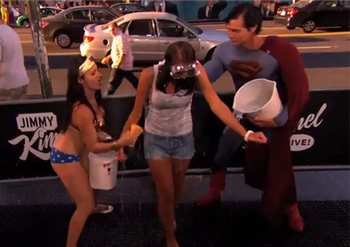
\includegraphics[width=3cm]{img/les5-gered1}

    
\includegraphics[width=3cm]{img/les5-gered2}
    \column{.5\textwidth}
    \centering
    
\includegraphics[width=3cm]{img/les5-gered3}

    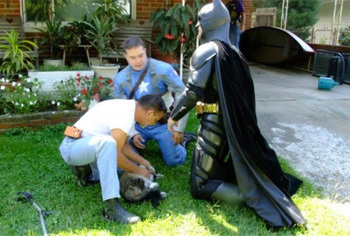
\includegraphics[width=3cm]{img/les5-gered4}
  \end{columns}

  \vfill
  \centering
  \small{Bron: \url{http://www.cracked.com/quick-fixes/4-people-who-saved-day-while-dressed-as-superheroes/}}
\end{frame}

\begin{frame}
  Stel, in een periode van 30 dagen werden er gemiddeld $3,483$ mensen per dag gered ($\overline{x}=3,483$, $n=30$)
  \vfill
  \begin{enumerate}
    \item Hypothese: $H_0: \mu = 3,3$; $H_1: \mu > 3,3$
    \item Significantieniveau: $\alpha = 0,05$
    \item Steekproefgrootheid: $\overline{x} = 3,483$
  \end{enumerate}
  \vfill
  Populatiestandaardafwijking (verondersteld gekend): $\sigma = 0,55$
\end{frame}

\begin{frame}
  \frametitle{Berekenen toetsingsgrootheid}
  
  \bigskip
  
  Uit centrale limietstelling volgt: $M \sim Nor(\mu = 3,3; \sigma = \frac{0,55}{\sqrt{30}}=0,1)$

  \centering
  \begin{tikzpicture}[scale=.8]
    \begin{axis}[domain=3.0:3.6, ymax=4.2, samples=100, enlargelimits=false ]
      \addplot [very thick,smooth,draw=hgblue] {gauss(3.3, 0.10041580220928045413)};
      \node [coordinate, pin={$\overline{x}= 3.483$}] at (axis cs: 3.483, 0){};
    \end{axis}
  \end{tikzpicture}
\end{frame}

\section{Overschrijdingskans}

\begin{frame}
  \frametitle{Overschrijdingskans}
  \alertbox{De \textcolor{hgyellow}{p-waarde} is de kans, indien de nulhypothese waar is, om een waarde te verkrijgen voor de toetsingsgrootheid die minstens even extreem is als de geobserveerde waarde.}

  \begin{itemize}
    \item $p$-waarde $< \alpha \Rightarrow$ $H_{0}$ verwerpen: de gevonden waarde voor $\overline{x}$ is te extreem;
    \item $p$-waarde $\geq \alpha \Rightarrow$ $H_{0}$ niet verwerpen: de gevonden waarde voor $\overline{x}$ kan nog verklaard worden door toeval.
  \end{itemize}
\end{frame}

\begin{frame}
  \frametitle{Overschrijdingskans}
  
  \bigskip

  \centering
  \begin{tikzpicture}[scale=0.6]
    \begin{axis}[domain=-3.5:3.5, ymax=0.42, samples=100, enlargelimits=false, clip=false ]
      \addplot [smooth, fill=black!20, domain=1.822:3.5] {gauss(0,1)} \closedcycle;
      \addplot [very thick,smooth,draw=hgblue] {gauss(0, 1)};
      \node  at (axis cs: 1.822, -.04){\small 1.822};
      \draw [-latex](axis cs:2.1,0.02) -- (axis cs:2.35,0.06);
      \node [text width=0.5cm] at (axis cs: 2.5, .095){$p= 0,0344$};
    \end{axis}
  \end{tikzpicture}
  
  \[ P(M > 3,483) = P \left(Z> \frac{3,483 - 3,3}{\frac{\sigma}{\sqrt{n}}}\right) = P (Z > 1,822) = 0,0344 \]
\end{frame}

\section{Kritieke gebied}

\begin{frame}
  \frametitle{Kritieke gebied}
  
  \bigskip
  
  \alertbox{Het \textcolor{hgyellow}{kritieke gebied} is de verzameling van alle waarden voor de toetsingsgrootheid waarbij de nulhypothese kan verworpen worden.}
  
  We zoeken een grenswaarde $g$ waarvoor geldt:
  \[ P(M > g) = \alpha \]

  Bepaal $z_\alpha$ waarvoor geldt:
  \[ P(Z > z_\alpha) = \alpha \Rightarrow g = \mu + z_\alpha . \frac{\sigma}{\sqrt{n}} \]
  
  \begin{itemize}
    \item Links van $g$: aanvaardingsgebied ($H_0$ niet verwerpen)
    \item Rechts van $g$: kritieke gebied ($H_0$ wel verwerpen)
  \end{itemize}
  
\end{frame}


\begin{frame}
  \frametitle{Kritieke gebied}

  \centering
  \begin{tikzpicture}
    \begin{axis}[domain=-3.5:3.5, ymax=0.42, samples=100, enlargelimits=false, clip=false ]
      \draw [-](axis cs:1.645,-0.03) -- (axis cs:1.645,0.06);
      \addplot [smooth, fill=black!20, domain=1.645:3.5] {gauss(0,1)} \closedcycle;
      \addplot [very thick,smooth,draw=hgblue] {gauss(0, 1)};
      \node [text width=0.8cm] at (axis cs: 1.645, -.06){$z_{\alpha}= 1.645$};
      \draw [-latex](axis cs:2.1,0.02) -- (axis cs:2.35,0.06);
      \node [text width=0.5cm] at (axis cs: 2.5, .095){$\alpha= 0.05$};
    \end{axis}
  \end{tikzpicture}

significantieniveau $\alpha = 0.05$ $\Rightarrow$ grenswaarde $z_{\alpha}$=1.645\\
($z_{\alpha} = $\texttt{qnorm(0.95)})
  
\end{frame}

\begin{frame}
  \frametitle{Linkszijdig toetsen}
  
  Wat zou je in de verg.  moeten veranderen opdat je de correcte kritieke waarde zou berekenen?
  \pause
  Antwoord:
  \[g = \mu \alert{-} z \times \frac{\sigma}{\sqrt{n}} \]
  want
  \[ P(M < g) = P\left(Z < \frac{g - \mu}{\frac{\sigma}{\sqrt{n}}}\right) = 0.05 \]
  
\end{frame}

\begin{frame}
\frametitle{Linkszijdig toetsen}
  Wegens de symmetrieregel kunnen we zeggen
  \[ P\left(Z > - \left( \frac{g - \mu}{\frac{\sigma}{\sqrt{n}}} \right) \right) = 0.05 \]
  
  De z-waarde die ermee overeen komt is 1.645 dus hebben we
  
  \begin{align*}
    z = \frac{-g + \mu}{\frac{\sigma}{\sqrt{n}}} &\Leftrightarrow -g = \frac{\sigma}{\sqrt{n}} z - \mu \\
    & \Leftrightarrow g = \mu - z \frac{\sigma}{\sqrt{n}}
  \end{align*}
  
\end{frame}

\begin{frame}
  \frametitle{Tweezijdig toetsen}
  Soms kan het ook zijn dat er tweezijdig moet getoetst worden. Er moeten dan twee kritieke grenswaarden berekend worden namelijk de linker- en de rechter grenswaarden.

\begin{equation}
  g = \mu \pm z \times \frac{\sigma}{\sqrt{n}}
  \label{eq:kritiekeGrenswaarde}
\end{equation}
\end{frame}

\begin{frame}
  \frametitle{Samenvatting}

\begin{table}
  \centering
  \begin{tabular}{l|ccc}
    \toprule
    Doel              & \multicolumn{3}{l}{\parbox{.7\textwidth}{Test op gemiddelde waarde $\mu$ van de populatie aan de hand van een steekproef van $n$ onafhankelijke steekproefwaarden}} \\
    \midrule
    Voorwaarde        & \multicolumn{3}{l}{\parbox{.7\textwidth}{De populatie is willekeurig verdeeld, $n$ voldoende groot}} \\
    \midrule
    Type test         & Tweezijdig           & Eenzijdig links & Eenzijdig rechts \\
    \midrule
    $H_{0}$           & $\mu = \mu_{0}$      & $\mu = \mu_{0}$ & $\mu = \mu_{0}$  \\
    $H_{1}$           & $\mu \neq \mu_{0}$   & $\mu < \mu_{0}$ & $\mu > \mu_{0}$  \\
    Verwerpingsgebied & $\left|z\right| > g$ & $z< -g $        & $z>g$            \\
    Teststatistiek    & \multicolumn{3}{c}{$z = \frac{\overline{x} - \mu_{0}}{\frac{\sigma}{\sqrt{n}}}$} \\
    \bottomrule
  \end{tabular}
  \caption{Samenvatting mogelijke toetsen}
  \label{tab:toetsingsprocedures}
\end{table}
\end{frame}

\section{Voorbeelden}

\begin{frame}
  \frametitle{Voorbeeld 1}
  Bij een aselecte steekproef van 50 waarnemingen vinden we volgende grootheden: gemiddelde $\overline{x} = 25$ en standaardafwijking s = $\sqrt{55} = 7.41$
  We willen weten of er reden is om aan te nemen dat gemiddelde van de populatie kleiner is dan 27.

\end{frame}

\begin{frame}
  \frametitle{Voorbeeld 1}
  
  \begin{description}
    \item[1] Bepalen van de hypothesen
    
      $H_{0} : \mu = 27$ en $H_{1}: \mu < 27$.
      
    \item[2] Vastleggen significantieniveau
    
      $\alpha = 0.05$ en $n=50$
      
    \item[3] Toetsingsgrootheiden \& waarde: steekproefgemiddelde $\overline{x} = 25$
    

  \end{description}
\end{frame}

\begin{frame}
  \frametitle{Voorbeeld 1 (vervolg)}

  \begin{description}
    \item[4a] Overschrijdingskans
    
    Volgens de centrale limietstelling geldt:
    
    \[ M \sim Nor(\mu = 27, \frac{\sigma}{\sqrt{n}}) \]
    \[ z = \frac{\overline{x} - \mu}{\frac{\sigma}{\sqrt{n}}} = \frac{25-27}{\sqrt\frac{55}{50}} \approx -1.91\]
    
    We vinden dus een overschrijdingskans van het gemiddelde $0.0281$.
    
    
    Bij een significantieniveau van 0.05 mogen we $H_{0}$ verwerpen.
  \end{description}

\end{frame}

\begin{frame}
  \frametitle{Voorbeeld 1 (vervolg)}

  \begin{description}

    \item[4b] Bereken en teken kritiek gebied
    
    \begin{align*}
    g &= \mu - z \times \frac{\sigma}{\sqrt{n}} \\
      &= 27 - 1.645 \times \sqrt{\frac{\sigma}{n}} \\
      &= 25.27470944
    \end{align*}

    We vinden dus dat $\overline{x} < g$ en dus kunnen we $H_{0}$ verwerpen.
  \end{description}
\end{frame}

\begin{frame}
  \frametitle{Voorbeeld 1 (vervolg)}
  
  \bigskip
  \centering
  \begin{tikzpicture}
    \begin{axis}[domain=24:30, samples=100, enlargelimits=false, clip=false ]
      \addplot [smooth, fill=cyan!20, domain=24:25.27] {gauss(27,1.048808848)} \closedcycle;
      \addplot [very thick,smooth,draw=hgblue] {gauss(27, 1.048808848)};
      \node  at (axis cs: 25.27, -.04){\small 25.27};
    \end{axis}
  \end{tikzpicture}
\end{frame}

\begin{frame}
  \frametitle{Voorbeeld 1 (vervolg)}
  
  \begin{description}
  
    \item[5] Conclusie
    
    We besluiten op basis van de steekproef dat $\mu < 27$ met een significantieniveau van $0,05$
  \end{description}
\end{frame}


\begin{frame}
  \frametitle{Voorbeeld 2}
  In een onderzoek naar het kleingeld dat in de zakken van  van  onze superhelden zit, wordt er van uit gegaan dat ze gemiddeld \euro{25} op zak hebben. We gaan ervan uit dat we een gekende spreiding van $\sigma = 7$ hebben. Verder zijn de gegevens van de aselecte steekproef van omvang $n=64$ beschikbaar met gemiddeld zakgeld $\overline{x}$ van \euro{23}. Neem als significantieniveau $\alpha = 0.05$.
\end{frame}

\begin{frame}
  \frametitle{Voorbeeld 2}
  
  \begin{description}
    \item[1] Bepalen van de hypothesen
    
      $H_{0} : \mu = 25$ en $H_{1}: \mu \neq 25$
      
    \item[2] Vastleggen significantieniveau
    
      $\alpha = 0.05$ en $n=64$.
      
    \item[3] Toetsingsgrootheden \& waarde: $\overline{x} = 23$
  \end{description}
  
\end{frame}

\begin{frame}
\frametitle{Voorbeeld 2 (vervolg)}

  \begin{description}
    \item[4b] Bereken kritieke gebied
    
    \[ g_{1} = \mu - z \times \frac{\sigma}{\sqrt{n}} = 23.28 \]
    \[ g_{2} = \mu + z \times \frac{\sigma}{\sqrt{n}} = 26.72 \]
    
    We vinden dat $\overline{x}$ in het kritieke gebied ligt (want $23 < 23.28$) dus mogen we $H_{0}$ verwerpen.
    \item[5] We kunnen op basis van deze steekproef besluiten dat de superhelden \textit{minder} dan \EUR{25} op zak hebben, met een significantieniveau van 5\%
  \end{description}
\end{frame}

\section{De $t$-toets}

\begin{frame}
  \frametitle{Veronderstellingen $z$-toets}
  
  
  \begin{itemize}
    \item De steekproef moet aselect zijn
    \item De steekproef moet voldoende groot zijn ($n \ge 30$)
    \item De variatie van de toetsingsgrootheid moet normaal verdeeld zijn
    \item We veronderstellen dat de standaardafwijking van de populatie, $\sigma$, gekend is
  \end{itemize}

  Als deze veronderstellingen niet gelden, mag je de $z$-toets niet gebruiken!
\end{frame}

\begin{frame}
  \frametitle{De $t$-toets}
  
  Bepalen kritieke grenswaarde:
  
  \[ g = \mu \pm t \times \frac{s}{\sqrt{n}} \]
  
  \begin{itemize}
    \item $t$-waarde wordt afgeleid uit de Student-$t$ verdeling, hangt af van aantal \textit{vrijheidsgraden}, $n-1$
    \item Op te zoeken in $t$-tabel of met R-functie \texttt{pt}
    \item Procedure hypothesetoets is verder identiek aan $z$-toets
  \end{itemize}
  
\end{frame}

\begin{frame}
  \frametitle{Vergelijken van twee steekproeven}
  
  Is steekproefgemiddelde van twee steekproeven significant verschillend?
  
  \begin{itemize}
    \item Onafhankelijke steekproeven
    \item Gepaarde steekproeven
  \end{itemize}
\end{frame}

\begin{frame}
  \frametitle{Onafhankelijke steekproeven}
  
  In een klinisch onderzoek wil men nagaan of een nieuw medicijn als bijwerking een verminderde reactiesnelheid heeft.
  
  \begin{itemize}
    \item Controlegroep: 6 deelnemers krijgen placebo
    \item Interventiegroep: 6 deelnemers krijgen medicijn
  \end{itemize}
  
  Vervolgens wordt reactiesnelheid gemeten:
  
  \begin{itemize}
    \item Controlegroep: 91, 87, 99, 77, 88, 91 ~~~~~~~~~~~($\overline{x}=88,83$)
    \item Interventiegroep: 101, 110, 103, 93, 99, 104 ~~($\overline{y}=101,67$)
  \end{itemize}
  
  Zijn er significante verschillen tussen de interventie- en controlegroep?
\end{frame}

\begin{frame}[fragile]
  \frametitle{Onafhankelijke steekproeven}
\begin{enumerate}
  \item Hypothese:
    \begin{itemize}
     \item $H_0$: $\mu_1 - \mu_2 = 0$
     \item $H_1$: $\mu_1 - \mu_2 < 0$
    \end{itemize}
  \item Significantieniveau: $\alpha = 0,05$
  \item Steekproefgrootheid:
    \begin{itemize}
     \item $\overline{x}-\overline{y} = -12,833$
     \item $\overline{x} =$ schatting voor $\mu_1$ (controlegroep) 
     \item $\overline{y} =$ schatting voor $\mu_2$ (interventiegroep) 
    \end{itemize}
\end{enumerate}
\vfill
In R:
{\footnotesize
\begin{Verbatim}[commandchars=\\\{\}]
> controle <-  c(91, 87, 99, 77, 88, 91)
> interventie <- c(101, 110, 103, 93, 99, 104)
> t.test(controle, interventie, alternative="less",
                                      mu=0, conf.level=0.95)
\end{Verbatim}
}
\end{frame}

\begin{frame}[fragile]
  \frametitle{Onafhankelijke steekproeven}

{\footnotesize
\begin{Verbatim}[commandchars=\\\{\}]
Welch Two Sample t-test

data:  controle and interventie
t = -3.4456, df = 9.4797, p-value = 0.003391
alternative hypothesis: true difference in means is less than 0
\sout{95 percent confidence interval:}      {\tiny \textcolor{red}{OPGELET!} Dit heeeft niets te maken met}
\sout{-Inf -6.044949}                       {\tiny   aanvaardingsgebied of kritiek gebied}
sample estimates:
mean of x mean of y 
88.83333 101.66667
\end{Verbatim}
}
\vfill
$\overline{x}-\overline{y}=-12,833$ komt overeen met $t=-3,4456$\\
$df=9,48$ wordt berekend door \texttt{t.test()} op basis van $x$ en $y$\\
$p = 0,003391 < \alpha = 0,05$ dus $H_0$ verworpen (significant verschil)
\end{frame}

\begin{frame}
  \frametitle{Gepaarde steekproef}
  
  In een studie werd nagegaan of auto's die rijden op benzine met additieven ook een lager verbruik hebben.
  
  Bij 10 auto's werd het verbruik gemeten (uitgedrukt in mijl per gallon) voor beide soorten benzine:
  
  \vspace{.5cm}
  \centering
  \begin{tabular}{|l|c|c|c|c|c|c|c|c|c|c|}
  	\hline
  	Auto           & 1  & 2  & 3  & 4  & 5  & 6  & 7  & 8  & 9  & 10 \\ \hline
  	Gewone benzine & 16 & 20 & 21 & 22 & 23 & 22 & 27 & 25 & 27 & 28 \\ \hline
  	Met additieven & 19 & 22 & 24 & 24 & 25 & 25 & 25 & 26 & 28 & 32 \\ \hline
  \end{tabular} 
\end{frame}

\begin{frame}[fragile]
  \frametitle{Gepaarde steekproef}
\begin{enumerate}
    \item Hypothese:
    \begin{itemize}
        \item $H_0$: $\overline{x-y} = 0$
        \item $H_1$: $\overline{x-y} > 0$
    \end{itemize}
    \item Significantieniveau: $\alpha = 0,05$
    \item Steekproefgrootheid:
    \begin{itemize}
        \item $\overline{x-y}$
        \item $x =$ mijl per gallon met additieven ($\overline{x}=25,1$)
        \item $y =$ mijl per gallon met gewone benzine ($\overline{y}=23,1$)
    \end{itemize}
\end{enumerate}
\vfill
In R:
{\footnotesize
    \begin{Verbatim}[commandchars=\\\{\}]
> gewone    <- c(16, 20, 21, 22, 23, 22, 27, 25, 27, 28)
> additieven <-c(19, 22, 24, 24, 25, 25, 26, 26, 28, 32)
> t.test(additieven, gewone, alternative="greater",
                      \textcolor{red}{paired=TRUE}, mu=0, conf.level=0.95)
    \end{Verbatim}
}
\end{frame}

\begin{frame}[fragile]
  \frametitle{Gepaarde steekproef}

{\footnotesize
\begin{Verbatim}[commandchars=\\\{\}]
Paired t-test

data:  additieven and gewone
t = 4.4721, df = 9, p-value = 0.0007749
alternative hypothesis: true difference in means is greater than 0
\sout{95 percent confidence interval:}      {\tiny \textcolor{red}{OPGELET!} Dit heeeft niets te maken met}
\sout{1.180207      Inf}                    {\tiny   aanvaardingsgebied of kritiek gebied}
sample estimates:
mean of the differences 
2
\end{Verbatim}
}
\vfill
$\overline{x}-\overline{y}=2$ komt overeen met $t=4,4721$\\
$p = 0,0007749 < \alpha = 0,05$ dus $H_0$ verworpen (significant verschil)
\end{frame}

\section{Fouten in hypothesetoetsen}

\begin{frame}
  \frametitle{Fouten in hypothesetoetsen}

  \begin{table}
    \centering
    \resizebox{\textwidth}{!}{%
      \begin{tabular}{@{}l|cc@{}}
        \toprule
        & \multicolumn{2}{c}{\textbf{Realiteit (onbekend)}} \\
        \textbf{Conclusie toets}          & \textbf{$H_{0}$ correct} & \textbf{$H_{1}$ correct}     \\
        \midrule
        \textbf{$H_{0}$ geaccepteerd}& Juist                    & Fout van type II \\
        \textbf{$H_{0}$ verworpen}   & Fout van type I          & Juist            \\
        \bottomrule
      \end{tabular}
    }
    \label{tab:hypfouten}
  \end{table}

  P(type I error) = $\alpha$ (= significantieniveau)
  
  P(type II error) = $\beta$
  
  $\beta$ berekenen is \textbf{\textit{niet}} triviaal, maar als $\alpha \searrow$ dan $\beta \nearrow$ 
\end{frame}

\section{Effectgrootte}

\begin{frame}
  \frametitle{Effectgrootte}
  
  \alertbox{De \textcolor{hgyellow}{effectgrootte} is een metriek die uitdrukt hoe groot het verschil tussen twee groepen is}
  
  \begin{itemize}
    \item Controlegroep vs. interventiegroep
    \item Kan je gebruiken naast hypothesetoets
    \item Vaak gebruikt in onderwijswetenschappen
    \item Er zijn verschillende definities, hier: \textit{Cohen's $d$}
  \end{itemize}
\end{frame}

\begin{frame}
\frametitle{Cohen's $d$}

\[ d = \frac{\overline{x_1} - \overline{x_2}}{s} \]

met $\overline{x_1}$, $\overline{x_2}$ gemiddelde van de steekproeven

en $s$ een gecombineerde standaardafwijking over beide groepen:

\[ s = \sqrt{\frac{(n_1 - 1) s_1^2 + (n_2 - 1) s_2^2}{n_1 + n_2 -2}} \]

met $n_1$, $n_2$ de steekproefgroottes, $s_1$, $s_2$ de standaardafwijking van beide groepen

\end{frame}

\begin{frame}
  \frametitle{Interpretatie Cohen's $d$}
  
  \begin{columns}
    \column{.5\textwidth}
    
    \begin{center}
      \begin{tabular}{ll}
        \toprule
        $|d|$  & \textbf{Effectgrootte} \\
        \midrule
        0,01 & zeer klein             \\
        0,2  & klein                  \\
        0,5  & matig                  \\
        0,8  & groot                  \\
        1,2  & zeer groot             \\
        2,0  & enorm                  \\
        \bottomrule
      \end{tabular}
    \end{center}
  
    \column{.5\textwidth}
    
    In onderwijswetenschappen (John Hattie):
    
    \begin{itemize}
      \item 0,4 = kantelpunt voor gewenste effecten
      \item effectgrootte $d = 1$: leerstof van 1j op 6m verwerken!
    \end{itemize}
  
    Zie bvb. \url{http://www.evidencebasedteaching.org.au/hatties-2017-updated-list/}
  \end{columns}
\end{frame}

\begin{frame}
  \frametitle{Typisch opzet onderzoek in onderwijs}
  
  \begin{itemize}
    \item Onderzoeksvraag: Is X een goede leerstrategie, m.a.w. heeft dit een positief effect op eindresultaten?
    \item Controlegroep gebruikt ``normale'', ``klassieke'' techniek
    \item In de interventiegroep wordt X toegepast
    \item Achteraf volgt evaluatiemoment
    \item Scores bepalen, $d$ berekenen
  \end{itemize}
\end{frame}

\end{document}
